\documentclass[t]{beamer}
\usepackage{helvet}
\usepackage{calc}
\usepackage[utf8]{inputenc}
\usepackage[english]{babel}

\usetheme{Ilmenau}

\setbeamercovered{transparent}
\setbeamertemplate{navigation symbols}{}

\usepackage{units}
\usepackage{amsbsy}
\usepackage{amsmath}
\usepackage{amssymb}
\usepackage{graphics}
\usepackage{graphicx}
\usepackage{epsf}
\usepackage{epsfig}
\usepackage{fixmath}
%\usepackage{pgfmath}
\usepackage{wrapfig}


\title{Closing Ceremony}
\subtitle{So long, and thanks for all the DPL-eating racoons}
\author{DebConf15 orga team}
\date{2015-08-21}

\begin{document}

% hide all subsections
\setcounter{tocdepth}{1}

\begin{frame}
	\titlepage
\end{frame}

\section{Numbers}

%\begin{frame}
%	\frametitle{Statistics}
%	\tableofcontents
%\end{frame}

\subsection{Infra \& Video}

\begin{frame}
	\frametitle{Infrastructure stats}
	\begin{itemize}
		\item Uplink speed 1 of Gbit/s
		\item One router, eight switches; later reduced to four switches with 10G links
		\item Two wireless LAN controllers, 32 Access Points
		\item Total bandwidth usage of about 4GB
		\item Peak bandwidth usage ~500Mbit/s
%		\item Passionate about FLOSS
	\end{itemize}
%	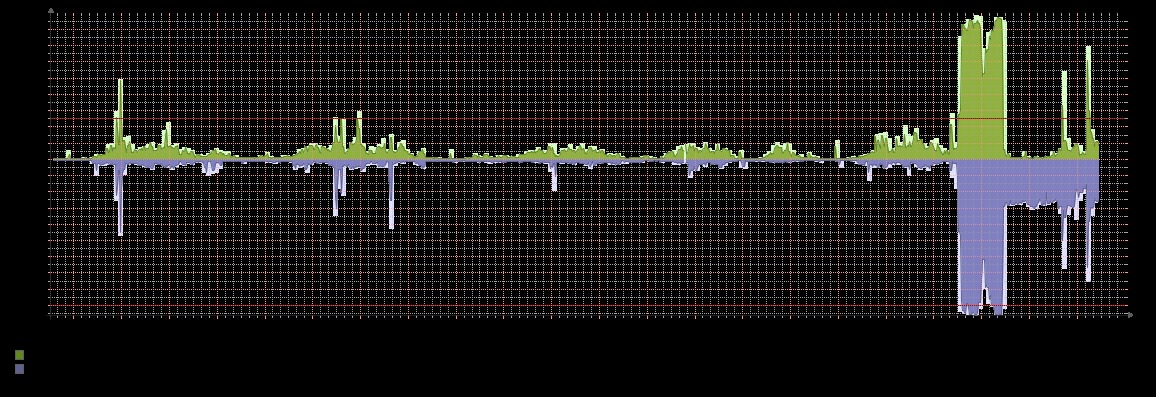
\includegraphics[scale=0.1]{weekly_traffic.jpg}
%	\begin{figure}
%		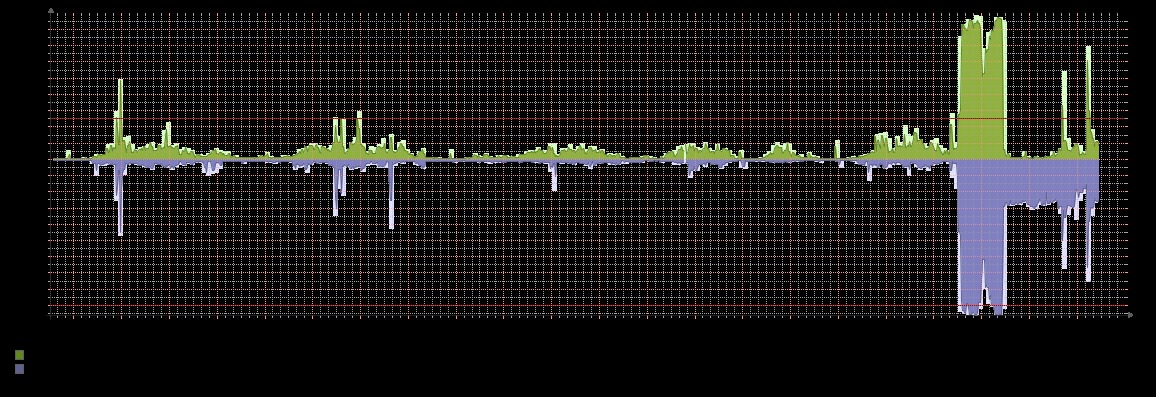
\includegraphics[scale=0.2,natwidth=1156,natheight=397]{weekly_traffic.jpg}
%	\end{figure}
\end{frame}

\begin{frame}
	\frametitle{Infrastructure problems}
	\begin{itemize}
		\item Three broken servers
		\begin{itemize}
			\item One of them kept us up until 03:30
		\end{itemize}
		\item Complete power outage in upstream data center
		\item "Interesting" pre-cabling structure within the building
		\begin{itemize}
			\item Ever burned through shoddy multi-mode cabling with 80 km reach single-mode 
		\end{itemize}
	\end{itemize}
\end{frame}

\subsection{Video Team}

\begin{frame}
	\frametitle{Video stats}
	\begin{itemize}
		\item video
		\item TODO
		\item TODO
	\end{itemize}
\end{frame}

\subsection{Misc}

\begin{frame}
	\frametitle{Food \& Drink}
	\begin{itemize}
		\item food \& drink
		\item TODO
		\item TODO
	\end{itemize}
\end{frame}

\begin{frame}
	\frametitle{Random}
	\begin{itemize}
		\item Number of badgers: 5
		\item Number of soaps: used: TODO, unused: 153
		\item Number of kids: TODO
		\item Number of beer cards: TODO
		\item Number of countries of origin: 55
		\item Number of registered attendees: 600+
		\item Number of : TODO
		\item Number of : TODO
	\end{itemize}
\end{frame}

\begin{frame}
	\frametitle{Child care}
	\begin{itemize}
		\item First DebConf with organized child care
		\item TecKids had a tech workshop for kids
		\item Increased need for quiet hacklabs
		\item Quoth the DPL: "this is a thing now"
	\end{itemize}
\end{frame}

\section{Future DCs}

\subsection{DebConf16}

\begin{frame}
	\frametitle{See you there?}
	\begin{itemize}
		\item Cape Town
		\item No raccoons, but penguins
		\item If you do work for Debian, but can't afford travel, please apply for travel sponsorship
		\item Also, penguins
	\end{itemize}
\end{frame}

\subsection{DebConf17}

\begin{frame}
	\frametitle{Three bids, already}
	\begin{itemize}
		\item Cambridge, United Kingdom
		\item Montreal, Canada
		\item Prague, Czech Republic
		\item You? Bids are still open!
		\item \url{https://www.debconf.org/wiki/DebConf17}
	\end{itemize}
\end{frame}


\section{Final information}

\subsection{}

\begin{frame}
	\frametitle{Announcements}
	\begin{itemize}
		\item Tip jars for the venue staff are outside of this room and at front desk
		\item Yes, you can put in unused drink vouchers %TODO
		\item If you give feedback via TODO, you are entering a raffle for another Chromebook, provided by HP
	\end{itemize}
\end{frame}

\begin{frame}
	\frametitle{Final raffle}
	\begin{itemize}
		\item Libreboot X200, provided by Meinberg
	\end{itemize}
\end{frame}


\section{Thank you}

\subsection{Sponsors}

\begin{frame}
	\frametitle{Platinum}
%	
\includegraphics[scale=1]{images/sponsors/platinum/hp.png}
%	
\includegraphics[scale=1,natwidth=300,natheight=123]{images/sponsors/platinum/hp.png}

%	\begin{itemize}
%		\item Physical Layer
%		\item Kabel
%		\item Kupfer, Wireless, Glas, etc
%	\end{itemize}
\end{frame}




\end{document}


%\begin{frame}
%	\frametitle{}
%	\begin{itemize}
%		\item 
%		\item 
%		\item 
%		\item 
%		\item 
%	\end{itemize}
%\end{frame}
